% concatenated from indeuqe.tex

\documentclass{article}
\usepackage{amsmath}
\usepackage{amssymb}
\usepackage{latexsym}
\usepackage{amsthm}
\usepackage{mathrsfs} 
\usepackage{wasysym}
\usepackage{fancyhdr}
\usepackage{xcolor}
\usepackage{amsfonts}
\usepackage{amssymb}
\usepackage{enumitem}
\usepackage{epsfig}
\usepackage{epstopdf}
\usepackage[normalem]{ulem}
\usepackage[T1]{fontenc}
\usepackage{eucal}
\usepackage{tikz}
\usepackage[utf8]{inputenc}
 

\renewcommand{\baselinestretch}{1.16}
\topmargin = -0.6 in \oddsidemargin = 0 in
\setlength{\textheight}{9in} \setlength{\textwidth}{6.5in}

% THEOREMS --------------------------------------------------------------
\newtheorem{thm}{Theorem}[section]
\newtheorem{cor}[thm]{Corollary}
\newtheorem{lem}[thm]{Lemma}
\newtheorem{prop}[thm]{Proposition}
\newtheorem{conj}[thm]{Conjecture}
\newtheorem{problem}[thm]{Problem}
\newtheorem{observation}[thm]{Observation}
\newtheorem{defn}[thm]{Definition}
\newtheorem{alg}[thm]{Algorithm}
\newtheorem{rem}[thm]{Remark}
\newcommand{\red}{\textcolor{red}}
\newcommand{\dist} {\mathrm{dist}}
\newcommand{\cir}{\mathrm{int}}
\newcommand{\idq}{{}^{\alpha}_{\omega}}

\title{Packing Independent Cliques in $K_4$-minor-free Graphs %and Subcubic Graphs
}

\author{Benjamin Xiao\thanks{Central Magnet School, Murfreesboro, TN 37132.} \ and \  Dong Ye\thanks{Department of Mathematics, Middle Tennessee State University, Murfreesboro, TN 37132.} }

\date{}
 

\begin{document}
\maketitle

\begin{abstract}
Let $G$ be a graph and $S$ be a set of cliques of $G$. The set $S$ is an indeque set if every component of $G[S]$, the subgraph induced by vertices of $S$, is a clique. In this paper, we prove that the indeque ratio of $K_4$-minor-free graphs is $\frac 1 2$, which settle two conjectures of Biro, Collado and Zamora. %Further, we provide a polynomial time algorithm to find the maximum indeque set of $K_4$-minor-free graphs. 
We also show that the indeque ratio of subcubic graphs is $\frac 1 2$. 
\end{abstract}
  
 
\section{Introduction}
All graphs considered in this paper are simple. A graph is {\em complete} if any two vertices of the graph are adjacent. A complete graph on $n$-vertex is denoted by $K_n$. 
 Let $G$ be a graph. A {\em clique} of $G$ is a complete subgraph. Let $S$ be a set of cliques of $G$, and let $G[S]$ denote the subgraph of $G$ induced by all vertices of $S$. 
A set $S$ of cliques is {\em independent} if every component of $G[S]$ is a clique, which is also called an {\em indeque set}. The {\em indeque number} of $G$ is defined as the maximum size of indeque sets, denoted by
\[\idq(G)= \max\{|S| : S\subseteq V (G) \mbox{ and } G[S]\mbox{ is a union of independent cliques}\}.\]


An indeque set of $G$ is also called an {\em independent set} or {\em stable set} if every clique in $S$ is a single vertex (i.e. $K_1$). The {\em independent number} of a graph $G$ is the cardinality of the largest independent set of $G$, denoted by $\alpha(G)$. The {\em clique number} of a graph $G$ is the cardinality of the largest clique of $G$, denoted by $\omega(G)$. As noted in~\cite{BCZ}, it holds that 
\[\max\{\alpha(G), \omega(G)\}\le\, \idq(G)\le \alpha(G)\cdot \omega(G).\] 
It is well-known that it is NP-complete to determine the  independent number of a planar graph (cf. \cite{AHU}). From Four-Color Theorem~\cite{RT}, every $n$-vertex plane graph $G$ has an independent set of size at least $n/4$, which implies $\idq(G)\ge n/4$. %If $G$ is a triangle-free plane graph, then $\idq(G)\le n/2$ as $\omega(G)\le 2$ for triangle-free graphs. 
For an $n$-vertex plane graph $G$, Biro, Collado and Zamora~\cite{BCZ} show $\idq(G) \ge 4n/15$ for an $n$-vertex planar graph, and further conjectured that $\idq(G)\ge 2n/5$ that is sharp if it holds. 

 An indeque set $S$ is called an {\em induced matching} if every clique is a single edge (i.e. $K_2$). The maximum size of an induced matching is denoted by $im(G)$. Hence it holds that $im(G)\le \idq(G)$.  Kanj et. al.~\cite{KPSX} proved that a 2-connected outerplanar graph $G$ with minimum degree two has a induced matching of size at least $n/2$, which implies that such an outerplanar graph $G$ has $\idq(G)\ge n/2$. It is NP-complete to determine $im(G)$ for planar graphs with maximum degree four~\cite{KS}, but the maximum induced matching problem can be solved in polynomial time for outerplanar graphs  (cf.~\cite{KK}). In general, it is hard to determine the indeque number of a graph even for planar graphs. For computational discussions, please refer to~\cite{ELWB}. 
 

\begin{defn}
    Let $\mathcal G$ denote a class of graphs. Define $$\idq(\mathcal G, n) = \min\{\idq(G) : G \in \mathcal G \mbox { and } |G| = n\}.$$
    Then, the \textit{indeque ratio} of $\mathcal G$ is defined to be $$\idq(\mathcal G) = \lim_{n \to \infty}\frac{\idq(\mathcal G, n)}{n}.$$
\end{defn}

For a given class of graphs $\mathcal G$, in order to find $\idq(\mathcal G)$, it needs to find a sharp lower bound of indeque number for this class of graphs. Salia et. al.~\cite{SSTZ} obtained that $\idq(\mathcal G, n)=(n+o(n))/\log_2(n)$ for the class $\mathcal G$ of comparability graphs of $n$-element posets with acyclic cover graph, which implies $\idq(\mathcal G)=0$. The indeque ratio has been studied for the class of plane graphs by Biro, Collado and Zamora~\cite{BCZ}, who prove that the indeque ratio of the class of forests as stated below.

\begin{thm}[Biro, Collado and Zamora, \cite{BCZ}]\label{thm:forest}
    Let $\mathcal F$ be the class of forests. Then 
    \[\idq(\mathcal F)=\frac 2 3.\]
\end{thm}

Biro, Collado and Zamora~\cite{BCZ} also proved the indeque ration of the class of graphs with path-width at most two is $1/2$, and they further made the following conjectures about the indeque ratio of the classes of series-parallel and outerplanar graphs. 

\begin{conj}[Biro, Collado and Zamora, \cite{BCZ}]\label{conj1}
    Let $\mathcal S$ be the class of series-parallel graphs. Then 
    \[\idq(\mathcal S)=\frac 1 2.\]
\end{conj}

\begin{conj}[Biro, Collado and Zamora, \cite{BCZ}]\label{conj2}
    Let $\mathcal O$ be the class of outerplanar graphs. Then
    \[\idq(\mathcal O)=\frac 1 2.\]
\end{conj}

As pointed out in~\cite{BCZ}, the indeque ratio of outerplanar graphs is at least $4/9$ which follows from the above theorem and a result of Hosono on maximum induced forests of outerplanar graphs~\cite{Ho}.  It follows directly from induced matching result of Kanj et. al.~\cite{KPSX} on outerplanar graphs that the indeque ratio for 2-connected outerplanar graphs with a minimum degree at least two is 1/2.


In this paper, we study the indeque ratio of $K_4$-minor free graphs. It is well-known that the $K_4$-minor-free graphs form a subclass of plane graphs. Along with this, Wald and Colbourn~\cite{WC} proved that $K_4$-minor-free graphs are equivalent to graphs with tree-width at most $2$. Hence the class of $K_4$-minor free graphs also include graphs with path-width at most two as a subclass. Both series-parallel graphs and outerplanar graphs are $K_4$-minor-free graphs. Every block of a $K_4$-minor-free graph is a series-parallel graph. The following is our main result.

\begin{thm}\label{thm:main}
Let $\mathcal K$ be the class of $K_4$-minor free graphs. Then
\[\idq(\mathcal K)=\frac 1 2 .\]
\end{thm}

Since $\mathcal O\subset \mathcal K$ and $\mathcal S\subset \mathcal K$, it follows that $\idq(\mathcal K)\le\idq(\mathcal O)$ and $\idq(\mathcal K)\le \idq(\mathcal S)$. Note that the $4$-cycle $C_4$ is a series-parallel and outerplanar graph which has $\idq(C_4)=2$. The union of disjoint $C_4$s shows that $\idq(\mathcal O)\le 1/2$ and $\idq(\mathcal S)\le 1/2$. Hence, Theorem~\ref{thm:main} settles Conjectures~\ref{conj1} and~\ref{conj2}. %We also provide a linear-time algorithm to find the maximum indeque set of a $2$-connected series-parallel graph, and a polynomial-time algorithm to compute the same for $K_4$-minor-free graphs. 
In the last section, we show that the class of subcubic graphs also has indeque ratio $1/2$. 

%In this paper, we plan to prove Theorem~\ref{thm:main}, then state a few algorithms for computing the maximum indeque set of any $K_4$-minor-free graph.

\section{$K_4$-minor-free graphs}

A graph is $K_4$-minor-free if it does not contain $K_4$ as a minor. It is well known that the $K_4$-minor-free graph contains two important subfamily of graphs: one is the family of outer-planar graphs and the other one is the family of series-parallel graphs. Duffin~\cite{D} revealed the connection between the $K_4$-minor-free graphs and the series-parallel graphs as follows.

\begin{thm}[Duffin~\cite{D}]\label{thm:parallel}
    A graph without cut-vertex is $K_4$-minor-free graph if and only if it is a series-parallel graph. 
\end{thm}

Hence, every block, defined as a maximal 2-connected subgraph, of a $K_4$-minor free graph is a series-parallel graph. The definition of a series-parallel graph is given as follows. 
A {\em 2-terminal graph} $G$ is a graph with two special vertices, called {\em source vertex $s$} and {\em sink vertex $t$}, denoted by $(G,s,t)$. A {\em series composition} of two 2-terminal graphs $(G_1,s_1,t_1)$ and $(G_2,s_2,t_2)$ is a new 2-terminal graph formed by $G_1$ and $G_2$ by identifying $t_1=s_2$ with source vertex $s_1$ and sink vertex $t_2$, denoted by $(G_1\bullet G_2, s_1, t_2)$. A {\em parallel composition} of two 2-terminal graphs $(G_1,s_1,t_1)$ and $(G_2,s_2,t_2)$ is a new 2-terminal graph formed by $(G_1, s_1,t_1)$ and $(G_2, s_2, t_2)$ by identifying $s_1$ and $s_2$ as the new source vertex $s$ and identifying $t_1$ and $t_2$ as the new sink vertex $t$, denoted by $(G_1\|G_2, s, t)$. A  graph is called a {\em series-parallel graph} if it can be constructed from $K_2$ by series and parallel compositions. A series-parallel graph can be recognized in linear time \cite{VTL}.

\begin{figure}[!htb]
\begin{center}
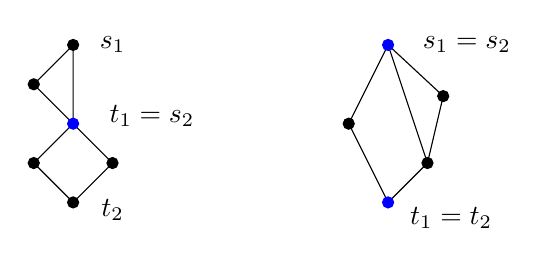
\begin{tikzpicture}
    \draw [](0,1) -- (-.5, .5)--(0,0)--(0,1);
    \draw [](0,0) -- (-.5,-.5)--(0,-1)--(.5, -.5)--(0,0);
    \filldraw[blue](0,0) circle (2pt);
    \filldraw[](0,1) circle (2pt);
    \filldraw[](0,-1) circle (2pt);
    \filldraw[](-.5,-.5) circle (2pt);
    \filldraw[] (.5,-.5) circle (2pt);
    \filldraw[] (-.5,.5) circle (2pt);
    \node at (1,0.1) {$t_1=s_2$};
    \node at (.5,1) {$s_1$ };
    %\node at (-1,-.5) {$v_3$ };
    \node at (.5,-1.1) {$t_2$ };

    \draw[](4,1) -- (3.5, 0) -- (4,-1);
    \draw[](4.5, -0.5)-- (4,1) -- (4.7, 0.35) -- (4.5, -0.5) -- (4,-1);
    \filldraw[blue](4,1) circle (2pt);
    \filldraw[](3.5,0) circle (2pt);
    \filldraw[blue](4,-1) circle (2pt);
    \filldraw[](4.7,0.35) circle (2pt);
    \filldraw[](4.5,-0.5) circle (2pt);

    \node at (5,1) {$s_1=s_2$};
    \node at (4.8, -1.2) {$t_1=t_2$};
\end{tikzpicture}
\caption{A series composition (Left) and a parallel composition (Right).}\label{fig1}
\end{center}
\end{figure}   

The following is the main result that we are going to prove.

\begin{thm}\label{thm:lower}
    Let $G$ be a $K_4$-minor-free graph. Then
    \[\idq(G)\ge  \frac 1 2 |V(G)|.\]
\end{thm}


Before proceeding to prove Theorem~\ref{thm:lower}, we need some terminologies that will be used throughout the proof. Let $G$ be a $K_4$-minor-free graph.  %For the proof of Theorem~\ref{thm:lower}, we focus on leaf-blocks of $G$. 
A {\em leaf-block} $H$ is block of $G$ sharing at most one vertex $v$ with other blocks of $G$, and the vertex $v$ is a cut-vertex separating $H-v$ and $G-H$ if it exists. 

Consider a leaf-block $H$ of a $K_4$-minor-free graph $G$. By Theorem~\ref{thm:parallel}, $H$ is a series-parallel graph. A maximal subgraph of $H$ constructed from $K_2$s by only series composition is called a {\em $0$-series-piece} of $H$. A $0$-series-piece of $H$ is a path of which every internal vertex has degree two in $G$. A maximal subgraph of $H$ with two terminals constructed from $0$-series-pieces by only parallel compositions is called a {\em $0$-parallel-piece}. A {\em $k$-series-piece} is a maximal subgraph constructed from $i$-parallel-pieces with $0\le i< k$ and $j$-series-pieces with $0\le j<k$ by only series compositions where at least one of these pieces is a $(k-1)$-parallel-piece. Then, a {\em $k$-parallel-piece} is a maximal subgraph constructed from $i$-series-pieces with $0\le i\le k$ and $j$-parallel-piece with $0\le j<k$ by only parallel compositions where at least one of these pieces is a $k$-series-piece. Note that a parallel-piece is 2-connected. For convenience, a $(k-1)$-parallel-piece is considered as a trivial $k$-series-piece, but a $k$-series-piece is not considered as a $k$-parallel-piece. A vertex of a $k$-series-piece or parallel-piece other than the two terminal vertices is called an {\em internal} vertex. %An internal vertex  and the vertex $v$ has the same degree in $G$. 


\begin{lem}[Eppstein, \cite{DE}]\label{lem:terminal}
Let $H$ be a 2-connected series-parallel graph. Then, for any edge $st$, $H$ is a 2-terminal graph with $s$ and $t$ as terminal vertices.
\end{lem}

For any $0$-series-piece $P$ of $H$ with terminal vertices $s$ and $t$, let $H'$ be a graph obtained from $H$ by replacing $P$ by an edge $st$. Then $H'$ is a 2-connected series-parallel graph. By Lemma~\ref{lem:terminal}, $H'$ is a 2-terminal graph with $s$ and $t$ as terminal vertices. Then $H$ is obtained from $H'-e$ and $P$ by a parallel composition. So $H$ is a 2-terminal graph with $s$ and $t$ as terminal vertices. So we have the following corollary.

\begin{cor}\label{cor:terminal}
Let $H$ be a 2-connected series-parallel graph. Then for any $0$-series-piece $P$ with terminal vertices $s$ and $t$, $H$ is a $k$-parallel-piece with terminal vertices $s$ and $t$ for some integer $k$. 
\end{cor}



In order to prove Theorem~\ref{thm:lower}, we consider a minimum counterexample $G$ with a leaf-block $H$. If $H$ has a subgraph $X$ that has an indeque set $S$ such that  $|S|\ge \frac 1 2 |V(X)|$ and every vertex of $S$ is not adjacent to any vertex in $G-X$, then any indeque set of $G-X$ together with $S$ form an indeque set of $G$. Note that $G-X$ is $K_4$-minor-free and has fewer vertices than $G$. As $G$ is a minimum counterexample, $G-X$ is not a counterexample and hence it has an indeque set $S'$ of size at least $\frac 1 2 |V(G-X)|$. So $S\cup S'$ is an indeque set of $G$. Therefore,
\[\idq(G)\ge |S\cup S'|=|S|+|S'|\ge \frac 1 2 |V(X)|+\frac 1 2 (|V(G)|-|V(X)|)=\frac 1 2 |V(G)|,\]
which leads a contradiction to that $G$ is a counterexample. Such a pair $(X, S)$ is called a {\em contra-pair} in the following. Hence, it suffices to show that $G$ always has a contra-pair.  



\begin{figure}[!htb]
\begin{center}
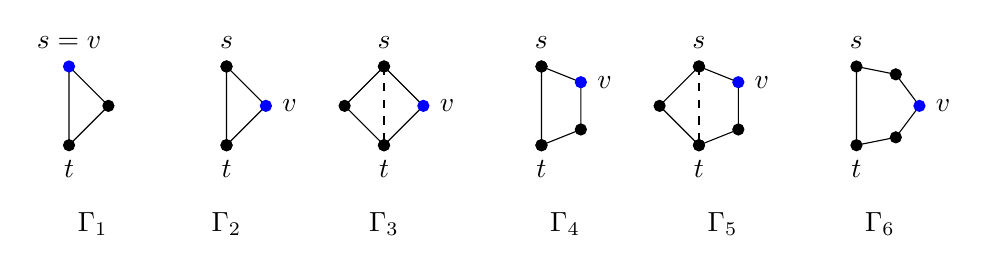
\begin{tikzpicture}
    \draw [](0,1) -- (.5, .5)--(0,0)--(0,1); \filldraw[] (.5,.5) circle (2pt);
%\node at (.8,.5) {$v$ };
  \node at (0,1.3) {$s=v$ };
    \node at (0,-.3) {$t$ };
\node at (.3, -1) {$\Gamma_1$};
 
    
    \draw [](2,1) -- (2,0)--(2.5, .5)--(2,1);
    \filldraw[ ](0,0) circle (2pt);
    \filldraw[blue](0,1) circle (2pt);
    \filldraw[](2,0) circle (2pt);
    %\filldraw[](1.5,.5) circle (2pt);
    \filldraw[blue] (2.5,.5) circle (2pt);
    \filldraw[] (2,1) circle (2pt);
    \node at (2.8,0.5) {$v$};
    \node at (2,1.3) {$s$ };
    \node at (2,-.3) {$t$ };
    \node at (2, -1) {$\Gamma_2$};

    \begin{scope}[shift={(2cm,0)}]
      \draw [](2,1) -- (1.5,.5)--(2,0)--(2.5, .5)--(2,1);
      \draw[dashed] (2,1)--(2,0);
    \filldraw[ ](0,0) circle (2pt);
    \filldraw[](0,1) circle (2pt);
    \filldraw[](2,0) circle (2pt);
    \filldraw[](1.5,.5) circle (2pt);
    \filldraw[blue] (2.5,.5) circle (2pt);
    \filldraw[] (2,1) circle (2pt);
    \node at (2.8,0.5) {$v$};\node at (2,1.3) {$s$ };
    \node at (2,-.3) {$t$ };
\node at (2, -1) {$\Gamma_3$};
    \end{scope}


    \begin{scope}[shift={(4cm,0)}]
      \draw [](2,1) --(2,0)--(2.5, .2)--(2.5,.8)--(2,1) ;
    \filldraw[ ](0,0) circle (2pt);
    \filldraw[](0,1) circle (2pt);
    \filldraw[](2,0) circle (2pt);
     
    \filldraw[blue] (2.5,.8) circle (2pt);
    \filldraw[] (2.5,.2) circle (2pt);
    \filldraw[] (2,1) circle (2pt);
    \node at (2.8,0.8) {$v$};\node at (2,1.3) {$s$ };
    \node at (2,-.3) {$t$ };
\node at (2.3, -1) {$\Gamma_4$};
    \end{scope}

     \begin{scope}[shift={(6cm,0)}]
      \draw [](2,1) -- (1.5,.5)--(2,0)--(2.5, .2)--(2.5,.8)--(2,1);
      \draw[dashed] (2,1)--(2,0);
    \filldraw[ ](0,0) circle (2pt);
    \filldraw[](0,1) circle (2pt);
    \filldraw[](2,0) circle (2pt);
    \filldraw[](1.5,.5) circle (2pt);
    \filldraw[blue] (2.5,.8) circle (2pt);
    \filldraw[] (2.5,.2) circle (2pt);
    \filldraw[] (2,1) circle (2pt);
    \node at (2.8,0.8) {$v$};\node at (2,1.3) {$s$ };
    \node at (2,-.3) {$t$ };
\node at (2.3, -1) {$\Gamma_5$};
    \end{scope}
    
   % \begin{scope}[shift={(8cm,0)}]
   %    \draw [](2,1) -- (1.5,.5)--(2,0)--(2.5, .5)--(2,1)--(2,0);
   % \filldraw[ ](0,0) circle (2pt);
   % \filldraw[](0,1) circle (2pt);
   % \filldraw[] (2,.5) circle (2pt);
   % \filldraw[](2,0) circle (2pt);
   % \filldraw[](1.5,.5) circle (2pt);
   % \filldraw[blue] (2.5,.5) circle (2pt);
   % \filldraw[] (2,1) circle (2pt);
   % \node at (2.8,0.5) {$v$};\node at (2,1.3) {$s$ };
   % \node at (2,-.3) {$t$ };
%\node at (2, -1) {$\Gamma_6$};

  %  \end{scope}

  

\begin{scope}[shift={(8cm,0)}]
      \draw [](2,1) --(2,0)--(2.5, .1)--(2.8,.5)--(2.5,.9)--(2,1) ;
      \filldraw[ ](0,0) circle (2pt);
    \filldraw[](0,1) circle (2pt);
    \filldraw[](2,0) circle (2pt);
     \filldraw[] (2.5,.9) circle (2pt);
    \filldraw[blue] (2.8,.5) circle (2pt);
    \filldraw[] (2.5,.1) circle (2pt);
    \filldraw[] (2,1) circle (2pt);
    \node at (3.1,0.5) {$v$};\node at (2,1.3) {$s$ };
    \node at (2,-.3) {$t$ };
\node at (2.3, -1) {$\Gamma_6$};
    \end{scope} 
    
\end{tikzpicture}
\caption{All possible 0-parallel-pieces with $v$ (edges in dashed lines may or may not be present).}\label{fig:0-parallel-piece}
\end{center}
\end{figure}   




\begin{lem}\label{lem:0-piece}
Let $G$ be a minimum counterexample to Theorem~\ref{thm:lower}, and let $H$ be a leaf-block of $G$ with a cut-vertex $v$. Then:

{\upshape (1)} $G$ does not contain two adjacent vertices of degree two, and hence every $0$-series-piece of $H$ is a path with at most three vertices if it does not contain $v$ as an internal vertex.

{\upshape (2)} every $0$-parallel-piece of $H$ is either a triangle or one of the six graphs containing $v$ in Figure~\ref{fig:0-parallel-piece} up to the symmetry exchanging $s$ and $t$. 
\end{lem}

\begin{proof}
Let $G$ be a $K_4$-minor-free graph with $\idq(G)<\frac 1 2 |V(G)|$ such that $|V(G)|$ is minimum, and let $H$ be a leaf-block with a cut-vertex $v$. \medskip 

(1) Suppose to the contrary that $G$ has two adjacent degree-2 vertices $v_1$ and $v_2$ different from $v$, and let $P:=v_3v_1v_2v_4$ (which could be a triangle). So $|V(P)|\le 4$. Then let $S=\{v_1,v_2\}$. So $S$ is an indeque set of $P$ and both $v_1$ and $v_2$ are not adjacent to any vertex of $G-P$. Hence $(P,S)$ is a desired contra-pair, a contradiction. So (1) holds. \medskip

(2) By Theorem~\ref{thm:parallel}, $H$ is a series-parallel graph. Note that all vertices of $H-v$ are not adjacent to any vertex of $G-H$.

Let $Q$ be a $0$-parallel-piece of $H$ with two terminals $s$ and $t$. Let $P$ be a $0$-series-piece in $Q$. Then every internal vertex of $P$ except $v$ has degree two in $G$. If $P$ does not contain $v$ as an internal vertex, then it follows from (1) that $|V(P)|\le 3$. If $P$ does contain $v$ as an internal vertex, then $|V(P)|\le 5$ and $|V(P)|=5$ if and only if $v$ is the middle vertex of $P$ by (1). So $Q-\{s,t, v\}$ is an independent set of $G$, denoted by $S$. So $(Q, S)$ is a contra-pair if $|S|\ge \frac 1 2 |V(Q)|$, which yields a contradiction. So $|S|<\frac 1 2 |V(Q)|$. 

If $v\in \{s,t\}$, then $|S|=|V(Q)|-2$. Therefore, $|V(Q)|-2=|S|<\frac 1 2 |V(Q)|$ which implies that $|V(Q)|\le 3$. Hence $Q$ is $\Gamma_1$. 

If $v\notin \{s,t\}$, then $|S|=|V(Q)|-3$. Therefore, $|V(Q)|-3<\frac 1 2 |V(Q)|$ which implies that $|V(Q)|\le 5$. If $v$ is not adjacent to $s$ or $t$, then $v$ is the middle vertex of a $0$-series-piece and $Q$ is $\Gamma_6$ in Figure~\ref{fig:0-parallel-piece} . If $v$ is adjacent to exactly one of $s$ and $t$, without loss of generality, assume $v$ is adjacent to $s$. It follows from (1) that $Q$ is either $\Gamma_4$ or $\Gamma_5$ in Figure~\ref{fig:0-parallel-piece}.  If $v$ is adjacent to both $s$ and $t$, then $v$ is not adjacent to any vertex of $S$. So consider $(Q-v, S)$ which is a contra-pair if $|S|\ge \frac 1 2 (|V(Q)|-1)$. Hence $|V(Q)|-3=|S|<\frac 1 2 (|V(Q)|-1)$ which implies that $|V(Q)|\le 4$. Therefore, $Q$ is either $\Gamma_2$ or $ \Gamma_3 $ in Figure~\ref{fig:0-parallel-piece}. So (2) follows. This completes the proof of the lemma. 
\end{proof}

 
A {\em triangle-string} is a series-parallel graph that can be constructed from a triangle-string by recursively performing one of the following two operations: (1) a parallel composition with a $K_2$, and (2) a series composition with a triangle.  
A {\em triangle-ring} is obtained from two triangle-strings by a parallel composition. 

Note that all $0$-parallel-pieces of  a  triangle-string or a triangle-ring are triangles. If one of the triangle of a triangle-string or a riangle-ring is replaced by some $\Gamma_i$ in Figure~\ref{fig:0-parallel-piece}, the resulting series-parallel subgraph is called a $\Gamma_i$-triangle-string or a $\Gamma_i$-triangle-ring. 



\begin{figure}[!htb]
\begin{center}
    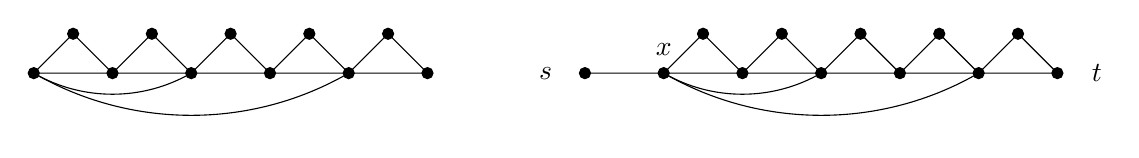
\begin{tikzpicture}
    \draw [](-2,0)--(-1.5,0.5)--(-1,0)--(-2,0);
    \draw [](-1,0)--(-0.5,0.5)--(0,0)--(-1,0);
    \draw [](0,0)--(0.5,0.5)--(1,0)--(0,0);
    \draw [](1,0)--(1.5,0.5)--(2,0)--(1,0);
    \draw [](2,0)--(2.5,0.5)--(3,0)--(2,0);
    %\draw [](3,0)--(3.5,0.5)--(4,0)--(3,0);
    %\draw [](4,0)--(4.5,0.5)--(5,0)--(4,0);
    \draw [](0,0) arc(-60:-120:2);
    \draw [](2,0) arc(-60:-120:4);
    \filldraw[](-2,0) circle (2pt);
    \filldraw[](-1,0) circle (2pt);
    \filldraw[](0,0) circle (2pt);
    \filldraw[](1,0) circle (2pt);
    \filldraw[](2,0) circle (2pt);
    \filldraw[](3,0) circle (2pt);
    %\filldraw[](4,0) circle (2pt);
    %\filldraw[](5,0) circle (2pt);
    \filldraw[](-1.5,0.5) circle (2pt);
    \filldraw[](-0.5,0.5) circle (2pt);
    \filldraw[](0.5,0.5) circle (2pt);
    \filldraw[](1.5,0.5) circle (2pt);
    \filldraw[](2.5,0.5) circle (2pt);
    %\filldraw[](3.5,0.5) circle (2pt);
   % \filldraw[](4.5,0.5) circle (2pt);

\begin{scope}[shift={(8,0)}]

   \draw [](-2,0)--(-1.5,0.5)--(-1,0)--(-2,0)--(-3,0);
    \draw [](-1,0)--(-0.5,0.5)--(0,0)--(-1,0);
    \draw [](0,0)--(0.5,0.5)--(1,0)--(0,0);
    \draw [](1,0)--(1.5,0.5)--(2,0)--(1,0);
    \draw [](2,0)--(2.5,0.5)--(3,0)--(2,0);
    %\draw [](3,0)--(3.5,0.5)--(4,0)--(3,0);
    %\draw [](4,0)--(4.5,0.5)--(5,0)--(4,0);
    \draw [](0,0) arc(-60:-120:2);
    \draw [](2,0) arc(-60:-120:4);
    \filldraw[](-2,0) circle (2pt);
    \filldraw[](-1,0) circle (2pt);
    \filldraw[](0,0) circle (2pt);
    \filldraw[](1,0) circle (2pt);
    \filldraw[](2,0) circle (2pt);
    \filldraw[](3,0) circle (2pt);
    \filldraw[](-3,0) circle (2pt);
    %\filldraw[](5,0) circle (2pt);
    \filldraw[](-1.5,0.5) circle (2pt);
    \filldraw[](-0.5,0.5) circle (2pt);
    \filldraw[](0.5,0.5) circle (2pt);
    \filldraw[](1.5,0.5) circle (2pt);
    \filldraw[](2.5,0.5) circle (2pt);
 
    \node at (-3.5,0) {$s$};
    \node at (3.5,0) {$t$ };
   \node at (-2,.3) {$x$ };
 

  
  
 %  \draw [](-2,0)--(-1.5,0.5)--(-1,0)--(-2,0);
 %   \draw [](-1,0)--(-0.5,0.5)--(0,0)--(-1,0);
  %  \draw [](0,0)--(0.5,0.5)--(1,0)--(0,0);
   %    \draw [](1,0)--(1.5,0.5)--(2,0)--(1,0);
    %   \draw [](2,0)--(2.5,0.5)--(3,0)--(2,0);
   %    \draw [](3,0)--(3.5,0.5)--(4,0)--(3,0);
     
  %     \draw [](0,0) arc(-60:-120:2);
  %     \draw [](2,0) arc(-60:-120:4);
  %     \draw [](4,0) arc(-60:-120:6);
   %    \filldraw[](-2,0) circle (2pt);
   %    \filldraw[](-1,0) circle (2pt);
   %    \filldraw[](0,0) circle (2pt);
  %     \filldraw[](1,0) circle (2pt);
   %    \filldraw[](2,0) circle (2pt);
  %     \filldraw[](3,0) circle (2pt);
   %    \filldraw[](4,0) circle (2pt);
   
  %     \filldraw[](-1.5,0.5) circle (2pt);
 %      \filldraw[](-0.5,0.5) circle (2pt);
  %     \filldraw[](0.5,0.5) circle (2pt);
  %     \filldraw[](1.5,0.5) circle (2pt);
  %     \filldraw[](2.5,0.5) circle (2pt);
 %      \filldraw[](3.5,0.5) circle (2pt);
   

\end{scope}
   
\end{tikzpicture}
\caption{A triangle-string (Left) and a kite (Right).}\label{fig2}
\end{center}
\end{figure}   



A {\em kite}  (or {\em $\Gamma_i$-kite}) is a series-parallel graph constructed from a $0$-series-piece $P$ (that is a path) and a  triangle-string ( or a  $\Gamma_i$-triangle-string). The terminal vertex of $P$ identified with a terminal vertex of the triangle-string (resp. $\Gamma_i$-triangle-string) is called the {\em joint vertex} of the kite (or $\Gamma_i$-kite). For example, see Figure~\ref{fig2} and $x$ is the joint vertex. 
  
In the following, we are going to prove Theorem~\ref{thm:lower}. 
 

\medskip
\noindent{\em \bf Proof of Theorem~\ref{thm:lower}.} 
    Suppose to the contrary that the statement does not hold and let $G$ be a counterexample with the minimum number of vertices. In the following, it suffices to prove that $G$ has a contra-pair, which leads to a contradiction.
     

If $G$ has a vertex $u$ of degree one, let $w$ be the unique neighbor of $u$. Then let $X=uv$ and $S=\{u\}$, and $(X, S)$ is a desired contra-pair.
 So assume that $G$ has no vertex of degree one. It follows that a vertex of $G$ is either a cut-vertex or belongs to a block. Let $H$ be a leaf-block of $G$. 


\medskip
\noindent{\bf Claim~1.} {\sl $H$ does not contain a triangle-ring or a $\Gamma_1$-triangle-ring.}
\medskip

\noindent{\em Proof of Claim~1.} If not, let $R$ be a triangle-ring or a $\Gamma_1$-triangle-ring. Let $S$ be the set of all degree-2 vertices of $R$. Then  $S$ is an independent set of $G$ and $|S|=\frac 1 2 |V(R)|$. Hence $(R, S)$ is a desired contra-pair, a contradiction. %The subgraph $G-V(R)$ is a $K_4$-minor-free graph with fewer number of vertices. By (i), $G-V(R)$ has an indeque set $S$ of size $|S|\ge \frac 1 2 |V(G)-V(R)|$. Note that $S\cup S'$ is an indeque set of $G$. So 
%\[\idq(G)\ge |S'\cup S|\ge \frac 1 2 (|V(G)|-|V(R)|)+\frac 1 2 |V(R)|=\frac 1 2 |V(G)|,\]
%which contradicts $\idq(G)<\frac 1 2 |V(G)|$. 
So the claim holds. 
\medskip

According to Claim~1, a parallel composition cannot be performed on two triangle-strings that do not include $v$ as an internal degree-2 vertex. By a similar argument and (1) of Lemma~\ref{lem:0-piece}, a parallel composition also cannot be applied to a triangle-string and a $0$-series-piece that does not include $v$ as an internal degree-2 vertex.


\medskip
\noindent{\bf Claim~2.} {\sl $H$ does not contain a kite that does not contain $v$ as an internal degree-2 vertex or its joint vertex.}
\medskip

\noindent{\em Proof of Claim~2.} If not, let $K$ be such a kite with $x$ as its joint vertex. If $K$ contains $v$, then $v$ is either the terminal vertex of $K$ or internal vertex of degree at least three. So $K$ may contain $\Gamma_1$ (or $\Gamma_1$-kite). Assume $K$ is formed by a $0$-series-piece $P$ and a triangle-string or $\Gamma_1$-triangle-string. Without loss of generality, assume $s$ is the terminal vertex of $K$ in $P$. By (1) of Lemma~\ref{lem:0-piece},  $P$ has at most three vertices. Let $K'=K-s$ if $P$ has three vertices and $K'=K$ if $P$ has exactly two vertices. 
%$K$ is formed by a $K_2$ and 
%Then $v\ne x$ could be an internal vertex of $K$ with degree bigger than two.  it follows from Lemma~\ref{lem:0-piece} that $K$ is either a kite or a $\Gamma_1$-kite. Without loss of generality, assume $K$ is formed by a $K_2$ and a triangle-string or $\Gamma_1$-triangle-string. 
Let $S:=\{\mbox{all degree-2 vertices of } K' \mbox{ except terminal vertices} \}\cup \{x\}$. Then $|S|=\frac 1 2 |V(K')|$, and all vertices of $S$ have no neighbors in $G-K'$. Therefore, $(K', S)$ is a desired contra-pair, a contradiction. 
Hence Claim~2 holds. 
\medskip

By Claim~2, a series composition cannot be performed on a triangle-string and a $0$-series-piece.  Let $H'$ be a $k$-series-piece or a $k$-parallel-piece not containing $v$ as an internal vertex. It follows from Lemma~\ref{lem:0-piece} that every $0$-parallel-piece of $H'$ is a triangle. By Claim~2, a series composition of $H'$ can only be applied to two triangle-strings, and by Claim~1, a parallel composition of $H'$ can only be applied to a $K_2$ and a triangle-string. Therefore, the following holds, \medskip
\begin{description}
\item ($*$) {\sl every $k$-series piece with $k\ge 1$ and every $k$-parallel piece with $k\ge 0$ not containing $v$ as an internal vertex is a triangle-string. }
 \end{description}
\medskip


First, assume that $v$ is contained in a $0$-parallel-piece $Q$ with terminal vertices $s$ and $t$. Then it follows from (2) of Lemma~\ref{lem:0-piece} that  $Q\in \{\Gamma_i | i\in [6]\}$. %Let $P$ be the $0$-series-piece of $Q$ containing $v$. 
By Corollary~\ref{cor:terminal}, $H$ is a 2-terminal graph with terminal vertices $s$ and $t$. Then either $H=Q$ or $H$ is obtained from $Q$ and $H'$ by a parallel composition where $H':=H-(Q-\{s,t\})$.

If $H=Q$, then $H=\Gamma_i$ for some $i$. It is easy to check that $H$ has an indeque set $S\subseteq V(H-v)$ with size $|S|\ge \frac 1 2 |V(H)|$. Hence $(H,S)$ is a desired contra-pair, a contradiction. So in the following, assume that $H\ne Q$ and hence it is obtained from $Q$ and $H'$ by a parallel composition. Note that $H'$ is not a $0$-series-piece because $H\ne Q$ (by the maximality of $0$-parallel-piece). So $H'$ is either a $k$-parallel-piece with $k\ge 0$ or a $k$-series-piece with $k\ge 1$. Since $v\notin H'$, it follows from ($*$) that $H'$ is a triangle-string. Therefore, $H$ is a $\Gamma_i$-triangle-ring. By Claim~1, $i\ne 1$. 


If $H$ is a $\Gamma_2$-triangle-ring, let the two neighbors of $v$ in $H$ be $v_1$ and $v_2$. Without loss of generality  assume $v_2$ is not a terminal vertex of $H$. Let $S=\{\mbox{all degree-2 vertices of } H\}\cup \{v_2\}$. Then $S$ is an indeque set of $H$ which are not adjacent to any vertices of $G-H$, and $|S|= \frac 1 2 |V(H)|$. So $(H,S)$ is a desired contra-pair. 

If $H$ is a $\Gamma_3$-triangle-ring. Let $S=\{\mbox{all degree-2 vertices of }H\}-\{v\}$ and then $ |S|= \frac 1 2 (|V(H)|-1)$.  Then $S$ is an independent set of $G$. So $(H-v, S)$ is a desired contra-pair. 

If $H$ is a $\Gamma_4$-triangle-ring, let $v_1$ be the neighbor of $v$ in $H$ that is a terminal vertex of $\Gamma_4$. Then all neighbors of $v_1$ belong to $H$. Let $S=\{\mbox{all degree-2 vertices of } H\}\cup \{v_1\}-\{v\}$, and $|S|= \frac 1 2 (|V(H)|+1)\ge \frac 1 2 |V(H)|$. Hence $(H,S)$ is a desired contra-pair. 

Now assume that $H$ is a $\Gamma_i$-triangle-ring for $i\in \{5, 6 \}$,  let 
$S=  \{\mbox{ all degree-2 vertices of } H \}-\{v\} $. Then $S$ is an independent set of $G$ and has size $|S|\ge \frac 1 2 |V(H)|$. Therefore, $(H,S)$ is a desired contra-pair, a contradiction. Hence $i\notin \{5,6\}$.  This contradiction implies that $v$ does not belong to a $0$-parallel-piece.  \medskip

So the smallest integer $k$ that a $k$-parallel-piece containing $v$ is at least 1. Assume that $v$ is contained in a $0$-series-piece $P$ with terminal vertices $s$ and $t$. Then $P$ has at most five vertices by (1) of Lemma~\ref{lem:0-piece}. By Corollary~\ref{cor:terminal}, $H$ is constructed from $P$ and a 2-terminal graph $H'$. Since $v$ is not contained in a $0$-parallel-piece, $H'$ is not a $0$-series-piece. 
It follows from ($*$) that $H'$ is a triangle-string. If $P$ has at least three vertices, then $H$ contains a kite or $\Gamma_1$-kite as described in Claim~2, a contradiction. So $P$ has exactly two vertices $s$ and $t$ and one of them is $v$.  Without loss of generality, assume $v=s$. %It follows from (1) of Lemma~\ref{lem:0-piece} that $P$ has at most three vertices. 
Let $S=\{\mbox{all degree-2 vertices of }H\}\cup \{t\}$. Then $S$ is an indeque set of $G$ and every vertex of $S$ is not adjacent to a vertex of $G-H$. Note that $|S|\ge \frac 1 2 |V(H)|$. Hence $(H, S)$ is a desired contra-pair. This completes the proof of Theorem~\ref{thm:lower}
\qed

%So assume that $v$ is an internal vertex of $P$. If $P$ has five vertices, then, by (1) of Lemma~\ref{lem:0-piece}, $v$ is the middle vertex of $P$. Let $S=\{\mbox{all degree-2 vertices of }H\}-\{v\}$. Then $S$ is an independent set of $G$ and $|S|=\frac 1 2 |V(H)|$. Note that every vertex of $S$ is not adjacent to a vertex of $G-H$. So $(H,S)$ is a contra-pair. If $P$ has four vertices, then  $v$ is adjacent to one of the terminal vertices of $P$, say $s$. Then let $S=(\{\mbox{all degree-2 vertices of }H\}-\{v\})\cup \{s\}$, which is an indeque set of $G$. Note that $|S|\ge \frac 1 2 |V(H)|$ and $(H,S)$ is a desired contra-pair. If $P$ has three vertices with $v$ as a middle one, then let $S=(\{\mbox{all degree-2 vertices of }H\}-\{v\})\cup \{s\}$ and $|S|=\frac 1 2 |V(H)|$. Since $S$ is an indeque set of $G$ and $S$ is not adjacent to any vertex of $G-H$, it holds that $(H, S)$ is a contra-pair, a contradiction. 



\medskip 

It follows from Theorem~\ref{thm:lower} that the indeque ratio of the class of $K_4$-minor-free graphs satisfies $\idq(\mathcal K) \ge \frac{1}{2}$. On the other hand, there are infinitely many $K_4$-minor-free graphs having indeque ratio $1/2$: for example, the 4-cycle and the triangle-rings etc. 
So $\idq(\mathcal K)\le \frac 1 2$. Therefore, $\idq(\mathcal K)=\frac 1 2$, and Theorem~\ref{thm:main} holds. 
 
 
 \iffalse

%%%%%%%%%%%%%%%%%%%%%%%%%%%%%
\section{Dynamic programming algorithm } 
%%%%%%%%%%%%%%%%%%%%%%%%%%%%%


The Indeque Set Problem, finding a maximum indeque set of a given graph, is equivalent to the Cluster Vertex Deletion problem, which is NP-hard~\cite{ELWB}.  
In this section, we provide a polynomial time algorithm to find a maximum indeque set for $K_4$-minor-free graphs. For series-parallel graphs, the algorithm can be improved to be completed in linear time steps. 


Let $G$ be a graph. A {\em tree decomposition} of a graph $G$ is  a tree $\mathcal T$ where each node/vertex $X$ of $\mathcal T$, denoted as a {\em bag}, is some subset $X \subset V(G)$, satisfying the following properties:
\begin{enumerate}
    \item[(i)] $\displaystyle \bigcup_{X \in \mathcal T}X = V(G)$.
    \item[(ii)] For all edges in $E(G)$, there exists a bag $X \in \mathcal T$ such that $G[X]$ contains this edge.
    \item[(iii)] For all $v \in V(G)$, the subtree of $\mathcal T$ induced by all bags $X$ that contain $v$ is connected.
\end{enumerate}
The {\em width} of a tree decomposition $\mathcal T$ is defined as \[\text{width}(\mathcal T):=\displaystyle \max_{X \in \mathcal T}(|X| - 1).\] Then, the {\em treewidth} of a graph $G$, denoted by $\text{tw}(G)$,  is the smallest value $k$ such that there exists a tree decomposition of $G$ with width $k$. Bodlaender~\cite{HLB} gave a linear time algorithm to find a tree decomposition $\mathcal T$ of $G$ with s treewidth  $\text{width}(\mathcal T)=\text{tw}(G)$. 

Let $G$ be a $K_4$-minor-free graph. Then $\text{tw}(G)\le 2$, and hence it has a tree-decomposition $\mathcal T$ such that each bag of $\mathcal T$ has size at most three. Such a tree-decomposition of $G$ can be found in linear time by Bodlaender's algorithm. Choose a vertex $X_0$ of $\mathcal T$ (a bag) as a root, then let $\mathcal L_i:=\{\text{ all bags }X \in \mathcal T | \text{dist}_{\mathcal T} (X_0, X)=i\}$ where $\text{dist}_{\mathcal T}(X_0,X)$ is the distance from $X$ to $X_0$ in $\mathcal T$. So $\mathcal L_0=\{X_0\}$ and $\mathcal L_1=N_{\mathcal T}(X_0)$ --- the neighborhood of $X_0$ in $\mathcal T$.  Let $t:=\max \{\text{dist}_{\mathcal T}(X, X_0) \ | \text{ all bags } X\in \mathcal T\}$. Then every bag in $\mathcal L_t$ is a leave of $\mathcal T$. Applying Bodlaender's tree decomposition algorithm to generate a tree-decomposition $\mathcal T$, pick a bag $X_0$ and then generate all layers $\mathcal L_i$ for $i=0, \ldots, t$. This process can be done in linear time. 

%A tree decomposition $\mathcal T$ of treewidth $k$ is {\em smooth} if all bags have size $k+1$ and two adjacent bags in $\mathcal T$ share exactly $k$ vertices of $G$. It is well-known that a tree decomposition from Bodlaender's algorithm can be efficiently converted to a smooth tree decomposition by adding vertices from the parent bag to a child bag and inserting bags if two adjacent bags having less number of common vertices. In order to find a maximum indeque set of a $K_4$-minor-free graph $G$, we start a smooth tree decomposition of $G$ with treewidth two.  The following is the detailed description of the algorithm.


\medskip
{\bf Finding Maximum Indeque Set in $K_4$-minor-free Graphs:}  \medskip

{\bf Input:}  \hspace{.25cm}  A $K_4$-minor-free graph $G=(V,E)$.

{\bf Output:} \ A maximum indeque set of $G$. \medskip

{\bf Algorithm:}  

Step 1: Apply Bodlaender's algorithm to generate a tree decomposition $\mathcal T$ with layers $\mathcal L_i$ with $i=0,\ldots, t$. 

Step 2: For each bag $X_{t,i}\in \mathcal L_t$, generate a list of all indeque sets of $X_{t,i}$. 


Step 3: Generate indeque sets for each bag in $\mathcal L_k$ with $k< t$: After generates a list of indeque sets for each bags in $\mathcal L_{k+1}$, move to bags in $\mathcal L_k$. For a bag $X_{k,i}\in \mathcal L_k$, find all neighbors of $X_{t,i}$ in $\mathcal L_{k+1}$, denoted by $X_{k+1, i_1},\ldots, X_{k+1, i_k}$. 

Step 4: if there is no bags left, we start from the bottom to merge these indeque sets to update their parents' indeque sets...

Step 5: 


\medskip










 






Considering $2$-terminal series-parallel graphs first, we define the {\em decomposition tree} of a $2$-terminal series-parallel graph $(G, s, t)$ to be a binary tree $T$ with three types of nodes: $\bullet$, $\parallel$, and $e$ nodes. The {\em $e$-nodes} are single edges or $K_2$, {\em $\bullet$-nodes} represent a series composition of graphs $G_1, G_2$ with children denoted as $T_1,T_2$ respectively, and {\em $\parallel$-nodes} represent a parallel composition of graphs $G_1, G_2$ with children also denoted as $T_1,T_2$ respectively. Note that root node of $T$ will always be $G$ and that $T$ is always a full binary tree. For the sake of brevity, we will say that any node in $T$ will also denote the respective subgraph of $G$. 

We now introduce a lemma that will be the basis of our recursive approach, then include a well-known proposition that is crucial in our complexity analysis.

\begin{lem}\label{lem:sp-op}
    If $(G_1, s_1, t_1)$ and $(G_2, s_2, t_2)$ are two-terminal series-parallel graphs joined by a parallel operation with $s_1 = s_2 = s$ and $t_1 = t_2 = t$, then $$\idq(G_1 \| G_2 - \{s, t\}) = \idq(G_1 - \{s_1, t_1\}) +\idq(G_2 - \{s_2, t_2\}).$$ Similarly, if they were joined by a series operation with $t_1 = s_2 = v$, then $$\idq(G_1 \cdot G_2 - \{v\}) = \idq(G_1 - \{t_1\}) +\idq(G_2 - \{s_2\}).$$
\end{lem}
\begin{proof}
    %For the parallel operation case, just note that $V(G_1) \cap V(G_2) = \{s, t\}$, immediately implying the result. Similarly, for the series operation case, just note that $V(G_1) \cap V(G_2) = \{v\}$, which also immediately implies the result.
    Note that $G_1\| G_2-\{s,t\}$ is the union of two disjoint subgraphs $G_1-\{s_1,t_1\}$ and $G_2-\{s_2,t_2\}$, and $G_1\cdot G_2-\{v\}$ the the union of two disjoint subgraphs $G_1-t_1$ and $G_2-s_2$. This proposition follows directly from the definition of the indeque number. 
\end{proof}

%\begin{prop}\label{prop:ev}
%    For any planar graph $G$ where $n = |V(G)|$ and $m = |E(G)|$, we must have that $m \leq 3n - 6$.
%\end{prop}

Building off of Lemma~\ref{lem:sp-op}, define a function $SPI(G, R)$ that will equal the size of the maximum indeque set of a two-terminal series-parallel graph $G$ with source vertex $s$ and sink vertex $t$ where $G$ is restricted by a weighting function $R: V(G) \to \{0,1,2,3\}$. For each vertex $v \in G$, $R(v)$ will be the parameter that restricts $v$ as follows: \begin{enumerate}
    \setcounter{enumi}{-1}
    \item No known restrictions are placed on $v$.
    \item $v$ is not in the indeque set.
    \item $v$ is in the indeque set but cannot induce into $G$, i.e. we do not allow any of $v$'s neighbors to also be included in the indeque set.
    \item $v$ is in the indeque set and can induce into $G$, i.e. we do allow $v$'s neighbors to be included in the indeque set.
\end{enumerate}

Along with this, define an indicator function 
\[I_R(v)=\begin{cases}
    1 & \text{if } R(v) > 1, \\
    0 & \text{otherwise}
\end{cases}\]

With all of the notation in place now, we can now prove one of our main results.

\begin{thm}\label{thm:sp-alg}
    Given that $(G, s,t)$ is a $2$-termimal series-parallel graph, the value of $SPI(G, R)$ is computable in $O(n)$ time for any choice of weighting function $R$ where $n = |V(G)|$.
\end{thm}
\begin{proof}
We will present an algorithm to compute this, then prove that said algorithm runs in linear time. First, construct the decomposition tree of $G$ and denote this as $T$. One modification we will make is at any $\parallel$-node in $T$ with respective graph $(G', s',t')$, if $s't'$ is an edge in $G'$, then the children of this node would be the edge $s't'$ and $G'$ without the edge $s't'$. Along with this, we will construct $T$ such that every $\parallel$-node will have at least one child that is either an $e$-node or a $\bullet$-node. Then, for every node $X \in T$, do the following:

Firstly, if $X$ is an $e$-node, then the domain of $R$ would have size $2$, which are the source and sink vertex. Then, if either $R(s) = 0$ or $R(t) = 0$, then set said value to $3$ in $R$ as we want the maximum possible indeque set. From here, we can compute the value of $SPI(X, R)$ depending on the values of unordered pair $(R(s), R(t))$ as $R(s)$ and $R(t)$ are interchangeable in $K_2$. These values are shown in Table~\ref{tab1} (Here, $-\infty$ denotes a sufficiently negative value so that any specific case is disregarded).
\begin{table}[!htb]
\begin{center}
\begin{tabular}{|l|l|l|l|l|l|l|}
\hline
$(R(s), R(t))$ & $(1,1)$ & $(1,2)$ & $(1, 3)$ & $(2,2)$ & $(2,3)$ & $(3,3)$ \\ \hline
$SPI(X, R)$    &   $0$   &   $1$   &   $1$    &$-\infty$&$-\infty$&   $2$   \\ \hline
\end{tabular}
\end{center}
\caption{Base case values}\label{tab1}
\end{table}

Then, if $X$ is a $\bullet$-node, then define $v$ to be the joining vertex of the two $2$-terminal subgraphs $(G_1, s,v)$ and $(G_2, v, t)$. Note that $X = G_1 \cdot G_2$ and that $v$ is a cut-vertex. From here, we have $3$ cases to consider. 
\begin{enumerate}[label=\textbf{Case \arabic*.},leftmargin=*]
\item If $R(v) = 1,2$, then because of how the restriction parameters are denoted above, we can essentially "remove" $v$ from $X$ and combine the two indeque sets of $G_1$ and $G_2$ under restrictions of $R$. Hence, we can set $SPI(X, R) = SPI(G_1, R) + SPI(G_2,R) - I_R(v)$ with the subtracted $I_R(v)$ accounting for possible overlap.
\item If $R(v) = 3$, then $v$ is in the indeque set and induces into $X$, so it can possibly induce into either $G_1$ or $G_2$. Because $v$ can only induce into one subgraph's indeque set, say $G_1$ as it is analogous otherwise, it must not induce into $G_2$'s indeque set, so no vertex in $N_{G_2}(v)$ can be in the same indeque set. Therefore, combining the two indeque sets would be a valid indeque set in $X$. To compute this, let $R' R$ except set $R'(v) = 2$, and set $$SPI(X,R) =\max(SPI(G_1, R) + SPI(G_2, R'), SPI(G_1, R') + SPI(G_2, R)) - 1,$$ subtracting $1$ to deal with the overlapping vertex $v$.
\item If $R(v) = 0$, then we have no information on $v$ at all. In that case, test $R(v) = 1, 2,3$, with each value being handled by the appropriate case above. Afterwards, set $SPI(X, R)$ to the maximum computed value.
\end{enumerate}

Otherwise, if $X$ is a $\parallel$-node, then denote the graphs joined by said composition as $(G_1, s, t)$ and $(G_2,s,t)$ where $X = G_1 \parallel G_2$. Then, we split into cases to compute $SPI(X, R)$.

\begin{enumerate}[label=\textbf{Case \arabic*.},leftmargin=*]
\item If $R(s), R(t) \neq 0,3$, then simply combining the two indeque sets of $G_1$ and $G_2$ under restrictions by $R$ creates a valid indeque set of $X$ under restrictions of $R$ by similar reasoning as in Case $1$ when $X$ is a $\bullet$-node. Hence, compute $$SPI(X, R) = SPI(G_1, R) + SPI(G_2, R) - I_R(s) - I_R(t),$$ subtracting $I_R(s)$ and $I_R(t)$ to account for overlap of terminal vertices with the indeque sets.

\item If $R(s) = 3, R(t) \neq 0,3$ (similarly if $R(t) \neq 3, R(s) = 3$), then by similar reasoning to Case $1$, we do not need to worry about $t$. Also by similar reasoning to Case $2$ when $X$ was a $\bullet$-node, $s$ can induce into either $G_1$ or $G_2$, and combining the indeque sets afterwards is a valid indeque set of $X$. To do this, let $R' = R$ except set $R'(s) = 2$. Afterwards, compute $$SPI(X, R) = \max(SPI(G_1, R) + SPI(G_2, R'), SPI(G_1, R') + SPI(G_2, R))  - I_R(s) - I_R(t),$$ with the subtracted values having the same reason as in Case 1.

\item If $R(s) = R(t) = 3$, then there $1$ special case to consider here, which we describe below.

If $\{s,t\}$ is an edge in $X$, then disregard the definition for $G_1, G_2$ above. Firstly, let $G_0$ be the graph of $X$ without the edge $\{s, t\}$. Let $v_1, v_2,\ldots,v_k \in X$ be all vertices such that $v_ist$ induces a $K_3$ in $X$ and $R(v_i) \neq 1, 2$ for all $1 \leq i \leq k$. Also, let $(P_i, s, v_i)$ and $(Q_i, v_i, t)$ denote the two-terminal series-parallel graph where $\{s,v_i\} \notin E(P_i)$ and $\{v_i,t\} \notin E(Q_i)$, and let $G_i$ be the subgraph of $G_{i - 1}$ that does not contain the path $sv_it$, $P_i$, and $Q_i$. We can see that $G_i, P_i, Q_i$ must be descendants of $G_{i - 1}$ in $T$. The tree structure will look like something in Figure~\ref{fig4}. % Possibility that G_i is the empty set, but it'll be easy to deal with
\begin{figure}[!htb]
\begin{center}
\begin{tikzpicture}
    [level distance=1cm,
     level 1/.style={sibling distance=6cm},
     level 2/.style={sibling distance=5cm}, 
     level 3/.style={sibling distance=3cm},
     level 4/.style={sibling distance=2cm},
     level 5/.style={sibling distance=2cm},
     level 6/.style={sibling distance=1cm}]
    \node {$\parallel = X$}
        child {node {$\parallel = G_0$}
            child {node {$\bullet$}
                child {node {$\parallel$}
                    child {node {$e=sv_1$}}
                    child {node {$P_1$}}
                }
                child {node {$\parallel$}
                    child {node {$e=v_1t$}}
                        child {node {$Q_1$}}
                }
            }
            child {node {$\vdots$}
                child {node {$\parallel = G_{i - 1}$}
                    child {node {$\bullet$}
                        child {node {$\parallel$}
                            child {node {$e=sv_i$}}
                            child {node {$P_i$}}
                        }
                        child {node {$\parallel$}
                            child {node {$e=v_it$}}
                            child {node {$Q_i$}}
                        }
                    }
                    child {node {$G_i$}}
                }
            }
        }
        child {node {$e=st$}};
\end{tikzpicture}
\caption{The structure of the decomposition subtree as described above}\label{fig4}
\end{center}
\end{figure}
    
On top of this, define $R_i: V(X) \to \{0,1,2,3\}$ to share the same mapping as $R$ except that $R_i(s) = R_i(v_i) = R_i(t) = 2$, and define $R'_i$ similarly except $R'_i(v_i) = 1$. Then, over all $1 \leq i \leq k$, we can compute $$SPI(G_i, R_i) + SPI(P_i, R_i) + SPI(Q_i,R_i) + \sum_{j = 1}^{i - 1}(SPI(P_j, R'_j) + SPI(Q_j, R'_j) - 2) - 3,$$ with the subtracted parts accounting for over-counted terminal vertices. %Meant to deal with a possible $K_3$.
    
After evaluating this special case, redefine $(G_1, s,t)$ and $(G_2, s,t)$ to be the two-terminal series-parallel graphs where $X = G_1 \parallel G_2$. As this case can be handled very similarly as in Case $2$ except on both terminal vertexes, let $R_0,R_1,R_2,R_3 = R$ where $R_0(s)=R_0(t)=R_1(s)=R_2(t)=2$ and $R_1(t)=R_2(s)=R_3(s)=R_3(t) = 3$. Finally, compute $$\max_{0\leq i\leq 3}(SPI(G_1, R_i) + SPI(G_2, R_{4-i}) - I_{R_i}(s) - I_{R_i}(t)).$$ %Extremely ugly way to represent this idea but I can't think of any better way.

Between both subcases, take $SPI(X, R)$ to be the maximum value that was computed.
\item If $R(s) = 0$ (similarly if $R(t) = 0$), then we can also test every other possible value of $R(s)$, those being $1, 2, 3$, evaluating their respective case as above (or repeat this case if $R(s) = R(t) = 0$). Then, we take $SPI(X, R)$ to be the maximum value.
\end{enumerate}

After applying the above to all nodes $X \in T$, the final value of $SPI(G, R)$ is the computed value when $X = G$, closing the algorithm.
 
We can see that the entire algorithm is a recursive brute force, with the union of the indeque sets of series-parallel subgraphs being possible because of similar arguments to Lemma~\ref{lem:sp-op}. Thus, it must follow that the computed value of $SPI(G, R)$ is correct.

Now, to determine the time complexity of this algorithm, let $n = |V(G)|$ and $m = |E(G)|$. Firstly, Valdes, Tarjan and Lawler~\cite{VTL} have shown that the decomposition tree $T$ can be constructed in $O(n)$ time. Note that this algorithm to construct $T$ is by reversing the construction of $G$. Regarding the modifications to $T$, the edge identification of terminal points is doable in constant time, so it will not affect the time complexity. By the noted observation, the second modification will also not affect the time complexity by simply appending the series/edge pieces joined by parallel composition to the tree one at a time. % will need to put something about the other modification, but I believe that it will not affect time complexity at all.

Because of the above modifications, we can see that any induced $K_3$ in $G$ can be found in a time complexity that scales linearly based on $|V(T)|$ by traversing this decomposition tree and looking for the tree structure shown in Figure~\ref{fig4}. Furthermore, in the special $K_3$ subcase, the above modification also guarantees that each subgraph mentioned in said case must appear as a node in $T$.

From here, as the number of different ordered pairs $(R(s), R(t))$ for source and sink vertices $s, t \in G$ is constant, we can now see that the number of unique $SPI$ computations that need to be done is directly proportional to $|V(T)|$. To compute the value of $|V(T)|$, note that $m$ is the number of leaves in $T$. Let $k$ be the number of inner nodes in the binary tree such that $|V(T)| = m + k$. Then, as each node in $T$ has either $0$ or $2$ children, we have that $$|V(T)| = 1 + \sum_{v \in T}\textnormal{children}(v) = 1 + 2k.$$

Equating the two gives that $m + k = 1 + 2k \implies k = m - 1$. By substituting this in, we obtain that $|V(T)| = 2m - 1$, implying that the remaining part of the algorithm must run in $O(m)$ time. Therefore, the total time complexity of the algorithm will be $O(n + m)$. However, as every simple $K_4$-minor-free graph is a simple planar graph, we have %by Proposition~\ref{prop:ev} 
that $O(n + m) = O(n)$, which completes the proof.
\end{proof}

As a direct corollary, we immediately have the following:
\begin{cor}
    There exists a linear-time algorithm to compute $\idq(G)$ where $(G, s,t)$ is a two-terminal series-parallel graph.
\end{cor}
\begin{proof}
    We must have that $\idq(G) = SPI(G, R)$ where $R \equiv 0$. By Theorem~\ref{thm:sp-alg}, this is computable in linear-time, so we are done.
\end{proof}

%Moving onto $K_4$-minor-free graphs, % We can simply do a bottoms-up approach starting from leaves I believe. Will also add more explanations to everything once I get the bones of the algorithm down. Nevermind the below does not work due to the fact that I overlooked something critical

%we can do a similar dynamic programming approach as above to compute $\idq(G)$.



\begin{thm}
    Given that $G$ is a $K_4$-minor-free graph, there exists an algorithm to compute $\idq(G)$ in $O(n^4)$ time where $n = |V(G)|$.
\end{thm}
\begin{proof}
    %Throughout the proof below, we will denote 
    Let $G$ be a given graph, and let $\mathcal C(G)$ be the set of all connected components of  $G$.

 Since $G$ is $K_4$-minor-free graph, it has a smooth tree decomposition $\mathcal T$ of width two. 
 
 Define a function $K_4I(X, W, R)$ to be the maximum indeque set of the graph corresponding to the subtree of $T$ with root $X$ under restrictions by both $W$ and $R$. $W$ is an indeque set of $G$ such that for all $C \in \mathcal{C}(W)$, $C \cap X \neq \emptyset$. Then, $R:\mathcal{C}(W)\to \{0, 1\}$ denotes the restriction parameter for each connected component $C \in \mathcal{C}(W)$ where $R(C) = 0$ means it cannot induce into $X$ and $R(C) = 1$ means the opposite. We can then see that $\idq(G) = K_4I(X_0, \emptyset,R)$ where $X_0$ is the root of $T$ and $R$ maps the empty set to $\{0, 1\}$. To compute this, we perform the following algorithm for all $X \in T$. % Will clean this up later for clarity

    Let $X' := X \cap W$. Then, let $S$ be some indeque set of $X - X'$ in $G$ such that $W' := W \cup S$ is also an indeque set of $G$. Furthermore, also check that for all $C \in \mathcal{C}(W)$ where $R(C) = 0$, we also have that $C \in \mathcal{C}(W')$. Note that there will be at most $2^{|V(X -X')|}$ possible sets for $S$.

    Now, for each $S$, let $X_1, X_2, \ldots, X_l$ be the children of $X$. Then, for every connected component $C \in \mathcal{C}(W')$ such that either $C \notin \mathcal{C}(W)$ or $R(C) = 1$, we will choose at most one $X_i$ such that $X_i \cap C \neq \emptyset$, and assign $C$ to only induce into $X_i$. Denote the set of all $C$ that induces only into $X_i$ as $\mathcal C_i$. Then, define $R_i:\mathcal{C}(W')\to \{0, 1\}$ to be a mapping where for every $C \in \mathcal{C}(W')$, $R_i(C) = 1$ if $C \in \mathcal C_i$ and $R_i(C) = 0$ otherwise.

    By setting it up as above, we can combine the indeque sets resulted from computing $K_4I(X_i, W', R_i)$ with $S$, which must then also be an indeque set in $G$. Hence, simply compute $$|S| + \sum_{i=1}^l(K_4I(X_i, W', R_i) - |S \cap X_i|),$$ with the overlap subtracted as to not overcount. Finally, set $K_4I(X, W, R)$ to be the maximum value over all possible $S$ and partitions of $\mathcal{C}(W')$ into $R_1, R_2, \ldots, R_l$. This closes the algorithm.

    We can see that this bottom-up recursive approach will check every single possible indeque set of $G$. Hence, as we are always returning the maximum value at every possible step, we must have obtained the value of $\idq(G)$ at the end of it all as there are only a finite number of nodes in $T$.

    To now compute the complexity of the algorithm, let $n = |V(G)|$. The first thing to consider is the computation of $T$ itself, which is well-known to be computable in linear time~\cite{HLB}. Next, as every $K_4$-minor-free graph is a partial $2$-tree, we must have that $|X| = 3$ for all $X \in T$ by definition. Thus, it follows that there will be at most $2^3 = 8$ possible subgraphs $S$. Along with that, the total number of possible pairs of $(W,R)$ is constant as well. Combining both of these, we have that $S$ will be computed in $O(1)$ time.

    From here, we can see that $\mathcal{C}(W') \leq 3$, with the inequality being sharp if $X$ was the graph of $3$ disjoint vertices all included in some component of $\mathcal{C}(W')$. Along with this, each connected component $C \in \mathcal{C}(W')$ will have at most $n - 1$ children nodes in $T$. Since $C$ has the option to also choose $X$ as the inducing node as well, $C$ has $n$ options in total. Hence, it then follows that this portion of the algorithm runs in at most $O(n^3)$ time to account for every single partition.\footnote{I could have included an AM-GM argument here to make the analysis more rigorous, but it only reduces the factor to $\frac{8}{27}n^3$, which does not change anything at all.}

    Finally, we have to run this computation over every single node $X \in T$, and we can easily see that $|T| = n - 2$. Thus, by combining everything together, we obtain a final time complexity of $O(n^3 \cdot n + n) = O(n^4)$, as desired. \footnote{I dislike that this never utilizes how the edges are constructed at all as in practice, almost every $X \in T$ would not be the set of $3$ disjoint vertices}
\end{proof}

%Moving onto $K_4$-minor-free graphs, we define the \em{block-cut tree} to be the decomposition of a graph $G$ into a tree $T$ with its nodes being the set of all blocks and cut-vertices of $G$. In the edge set of $T$, a block $B \in G$ and a cut-vertex $v \in G$ have an edge between them if and only if $v \in B$. It is well-known that any connected graph has a block-cut tree. For the sake of clarity, we will be referring to the node in $T$ and the respective subgraph in $G$ interchangeably.

%By considering the block-cut tree $T$ of a $K_4$-minor-free graph $G$, we can see that by Theorem~\ref{thm:parallel} that every block node $B \in T$ must be a $2$-connected series-parallel graph. Hence, this leads to the following.

%\begin{thm}
%    For any $K_4$-minor-free graph $G$, there exists a linear-time algorithm to compute $\idq(G)$.
%\end{thm}
%\begin{proof}
%Let $T$ denote the block-cut tree of $G$, and let $S$ denote the set of all cut-vertex nodes in $T$. Then, let $W: S \to \{0,1,2,3\}$ be another weighting function such that for all $v\in S$, $W(v)$ represents the restriction parameter of $v$. The parameters will be the same ones as denoted above.

%Now, define a function $K_4I(T, W)$ as the maximum indeque set of a $K_4$-minor free graph corresponding to block-cut tree $T$ with restrictions placed on the set of cut-vertex nodes $S$ by $W$. Then, we must have that $\idq(G) = K_4I(T, W)$ where $W \equiv 0$. It then suffices to show that a linear-time algorithm to compute $K_4I(T, W)$ for any choice of $T,W$, which we will do below.

%Firstly, if there exists a leaf node $B \in T$ that is a leaf-block, then let $v \in T$ denote the adjacent node to $B$ in $T$. Then, let $R:V(B)\to \{0,1,2,3\}$ denote the weighting function on the vertices of $B$. Now, if there does not exist any $v$, then we trivially have that $K_4(T, W) = SPI(B, R)$. Otherwise, there are $3$ cases to consider:
%\begin{enumerate}[label=\textbf{Case \arabic*.},leftmargin=*]
%\item If $W(v) = 1, 2$, then set $R(v) = W(v)$. From here, we can see that $$K_4I(T, W) = K_4I(T - B, W) + SPI(B, R) - I_W(v)$$ with the subtracted part to account for possible overlap of vertices.
%\item If $W(v) = 3$, then we either have that $v$ induces into leaf-block $B$ or the remainder of the block-cut tree $T - B$. Hence, we can consider both cases by letting $R(v) = 2$, then defining $R' = R, W'=W$ where $W'(v) = 2$ and $R'(v) = 3$. Finally, we must have that $$K_4I(T, W) = \max\{K_4I(T-B, W)+SPI(B, R),K_4I(T-B, W')+SPI(B, R')\} - 1$$ with the subtracted parts to similarly account for the overlapping vertex $v$.
%\item If $W(v) = 0$, then just check all other possible values of $W(v)$ (those also being $1, 2, 3$), and evaluate each case as above. Then, set $K_4I(T, W)$ as the maximum computed value.
%\end{enumerate}

%Otherwise, we can see that every single leaf node of $T$ must be a cut-vertex node. Then, choose one of these leaf nodes and let $B \in T$ be the adjacent block to said node. Now let $v_1, v_2, \ldots, v_k \in T$ denote the cut-vertex leaves that are adjacent to $B$. Then, by defining $R:V(B) \to \{0,1,2,3\}$ to be the weighting function on $B$, we can set $R(v_i) = W(v_i)$ for all $1 \leq i \leq k$. Finally, we can remove $v_1, v_2, \ldots, v_k$ from $T$ and treat this case similarly to above as $B$ would now be a leaf-block in the modified $T$. This closes the algorithm. 

%We can trivially see that this whole algorithm is also a recursive brute force, so the computed value for $K_4I(T, W)$ must be correct. %May need to add onto this

%To analyze the time complexity, let $n = |V(G)|$. Firstly, the computation of the block-cut tree $T$ is well-known to be doable in $O(n)$ time. Then, as we are computing $SPI$ for every block $B \in T$, we have by Theorem~\ref{thm:sp-alg} that this is computable in $O(|V(B)|)$ time. Summing over every single block then gives that every $SPI$ computation runs in $O(n)$ time as the number of cut-vertices (the overlap between $SPI$ computations) is linearly upper-bounded by $n$.

%Now analyzing $K_4I$, as there is a constant number of cases, we can see that the number of distinct $K_4I$ computations will linearly scale with the size of $V(T)$. This can easily been seen to be upper-bounded by $n$, so this part of the algorithm must also run in $O(n)$ time complexity.

%Combining both of these together, we get that the total time complexity must be $O(n)$, so we do have a linear time algorithm to compute $K_4I(T, W)$ for any choice of $W$, as desired.
%\end{proof}
\fi

\section{Concluding Remarks}

A {\em subcubic graph} is a graph with maximum degree at most three. Hsieh, Le, Le and Peng~\cite{HLLP} recently show that it is NP-complete to determine the indeque number of subcubic planar graphs (Cluster Vertex-Deletion or 2-Claw Vertex-Deletion Problem, see Theorem~2 in \cite{HLLP}). It is also NP-complete to determine the inducing matching number of subcubic planar graphs~\cite{HOV}. In~\cite{KMM}, Kang, Mnich and M\"uller provided a polynomial-time algorithm to find an induced matching of size at least $m/9$ in a subcubic planar graph with $m$ edges.  

The following result gives a sharp lower bound for indeque number of subcubic graphs, and consequently  the indeque ratio of  subcubic graphs.

\begin{thm}
Let $G$ be an $n$-vertex subcubic graph. Then 
\[\idq(G)\ge \frac n 2,\]
and the bound is sharp. 
\end{thm}
\begin{proof}
    Let $G$ be a subcubic graph. Let $(X,Y)$ be a vertex partition of $G$ that maximizes the size of $E(X,Y)$, the set of edges joining a vertex of $X$ and a vertex of $Y$. If one part of $(X,Y)$, say $X$, has a vertex $v$ with degree at least two neighbors in its own part $X$. Then the partition $(X\backslash \{v\}, Y\cup \{v\})$ is a new vertex partition and 
    \[|E(X\backslash \{v\}, Y\cup \{v\})|>|E(X,Y)|,\] which contradicts that the maximality of $|E(X,Y)|$. Therefore, every vertex of $X$ or $Y$ has at most one neighbor in its own part, which means the vertex-induced subgraphs $G[X]$ and $G[Y]$ have maximum degree at most one. 
    Hence both $X$ and $Y$ are indeque sets of $G$. Note that $|X|+|Y|=|V(G)|=n$. It follows 
    \[\idq(G)\ge \max\{|X|, |Y|\}\ge \frac n 2.\]
    This completes the proof of the first part.
    
    To see the sharpness, there are 2-connected subcubic graphs with $4k$ vertices having indeque number $2k$: consider the subcubic graphs constructed from a cycle by blowing up every vertex to a square. It is quite easy to see that the graph has an indeque set of size $2k$. The graph does not have an indeque set of size at least $2k+1$. Otherwise, one of the 4-cycles contains at least three vertices from the indeque set, which is impossible because a 4-cycle has an indeque number two. 
\end{proof}

It follows immediately that the indeque ratio of all subcubic graphs is $1/2$. 

\begin{thm}
Let $\mathcal C$ be the class of all subcubic graphs. Then the indeque ratio of $\mathcal C$ is 
\[\idq(\mathcal C)=\frac 1 2.\]
\end{thm}

Note that the 3-dimensional hypercube $Q_3$ has indeque number 4. As noted by Biro, Collado and Zamora~\cite{BCZ}, the indeque ratio of any class $\mathcal G$ of graphs is closed under disjoint union.  Hence the indeque ratio for cubic graphs is also $1/2$.  

It was conjectured by Biro, Collado and Zamora~\cite{BCZ} that the indeque ratio of plane graphs is $2/5$. Note that, $K_4$-minor-free graphs, subcubic graphs and plane graphs have small maximum average degree. It is interesting to study the family of graphs with bounded maximum average degree. 

%The density of a graph $G$ is defined as $d(G)=|E(G)|/|V(G)|$. The density of $K_4$-minor-free graphs is at most 2, and the density of subcubic graphs $G$ is at most $3/2$, and the density of planar graphs is at most $3$. It is natural to ask what the indeque ratio could be for  graphs with bounded densities. 


%\begin{conj}
%Let $G$ be an $n$-vertex graph. Then 
%\[\idq(G)\ge \frac {2n} 5.\]
%\end{conj}


\begin{thebibliography}{00}
\parskip=-0.05cm
\bibitem{AHU} A.V. Aho, J.E. Hopcroft, and J.D. Ullman, The Design and Analysis of Computer Algorithms, Addison-Wesley, Reading, MA (1974).

\bibitem{BCZ} C. Biro, G. Collado and O. Zamora, Packing independent cliques into plane graphs, Theory \& Appl. Graphs, 12 (2) (2025) \# 3.

%\bibitem{HLB} H.L. Bodlaender, A linear time algorithm for finding tree-decompositions of small treewidth, SIAM J. Comput. 25 (6) (1996), 1305-1317

\bibitem{D} R.J. Duffin, Topology of series‐parallel networks, J. Math. Anal. Appl., 10 (1965) 303--318.

\bibitem{DE} D. Eppstein, Parallel recognition of series–parallel graphs, Inform. \& Comput., 98 (1) (1992) 41--55.

\bibitem{ELWB} Z. Ertem, E. Lykhovyd, Y. Wang and S. Butenko, The maximum independent union of cliques problem: complexity and exact approaches. J. Global Optim., 76 (3) (2020) 545--562.

\bibitem{HOV} H. Hocquard, P. Ochem and P. Valicov, Strong edge-colouring and induced matchings, Inf. Process. Lett., 113 (19-21) (2013) 836--843.
 
\bibitem{Ho} K. Hosono, Induced forests in trees and outerplanar graphs, Proc. Fac. Sci. Tokai Univ., 25 (1990) 27--29.

\bibitem{HLLP} S.-Y. Hsieh, H.-O. Le, V.B. Le, and S.-L. Peng, On the $d$-claw vertex deletion problem, Algorithmica, 86 (2) (2024) 505--525.

\bibitem{KMM} R.J. Kang, M. Mnich and T. M\"{u}ller, Induced matchings in subcubic planar graphs, SIAM J. Discrete Math., 26 (3) (2012) 1383--1411.

\bibitem{KPSX} I. Kanj, M.J. Pelsmajer, M. Schaefer and G. Xia, On induced matching problem, J. Comput. \& Sys. Sci., 77 (6) (2011) 1058--1070.

\bibitem{KS} C.W. Ko, F.B. Shepherd, Bipartite domination and simultaneous matroid covers, SIAM J. Discrete Math., 16 (2003) 517--523.

\bibitem{KK} A. Kostochka, J. Kratochvil, Covering and coloring polygon-circle graphs, Discrete Math., 163 (1997) 299--305.

\bibitem{SSTZ} N. Salia, C. Spiegel, C. Tompkins and O. Zamora, Independent chains in acyclic posets, arXiv: 1912.03288v2 (2019). 

\bibitem{RT} R. Thomas, An update on the Four-Color Theorem, Notices Am. Math. Soc. 45 (7) (1998) 848–859.

\bibitem{WC} J.A. Wald and C.J. Colbourn, Steiner trees, partial 2‐trees, and minimum IFI networks, Networks 13 (1983) 159–167.

\bibitem{VTL} J. Valdes, R.E. Tarjan, E.L. Lawler, The recognition of series parallel digraphs. SIAM J. Comput. 11 (2) (1982), 298--313.

\end{thebibliography}




\end{document}
